\section{Target and Detectors}
COMPASS experiment comprises large number of detectors, for identifying and measuring the particles coming out of interaction vertices. There are also detectors which monitor the particle beams and trigger other components to decide when the signals should be read out or not. In this section, the basic functionalities of different kinds of detectors are introduced in a simple manner. 

\begin{figure*}[!ht]
	\centering
	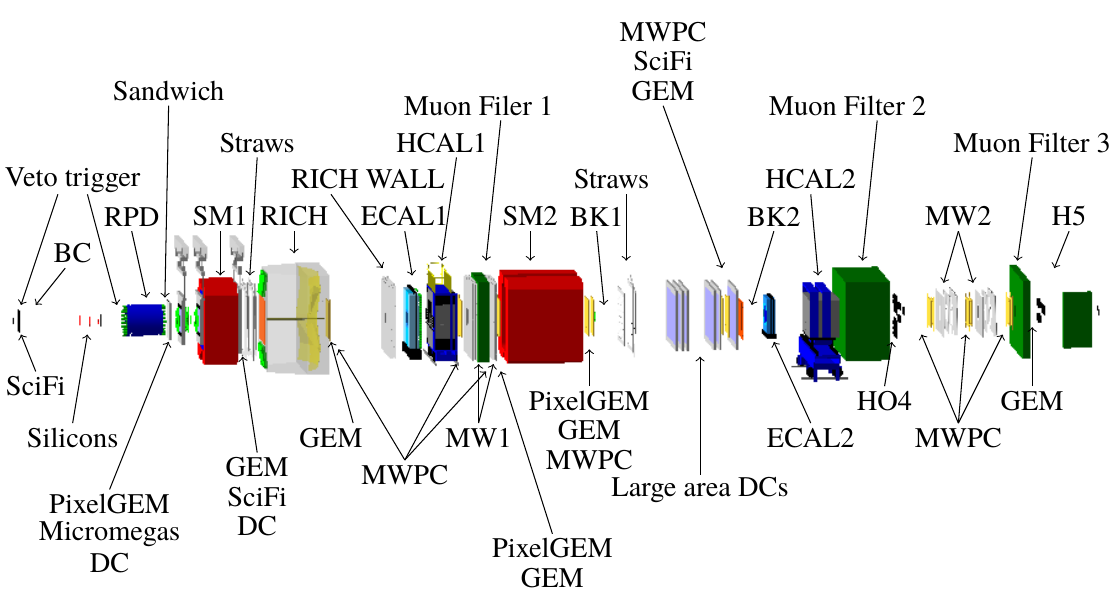
\includegraphics[width=\textwidth]{detector_layout}
	\caption{The layout of COMPASS detectors. The length of whole setup is around 50 meters. Pion beam comes from the left side of detectors and hits the target, which is surrounded by recoil-proton detector (RPD). On the right side of target, two different sets of detectors are used to measure out-going particles with small and large scattering angles.}
	\label{fig:detec_layout}	
\end{figure*}

\subsection{Particle beam and target}
To create the projectile particle beam, the proton beam, which is accelerated by the Super Proton Synchrotron (SPS), is firstly directed into Beryllium. From the nuclear reaction between proton and Beryllium nucleus, a secondary hadron particle beam is created, which is the incoming particle beam for the scattering experiment. In this project, the hadron beam is selected to be negative charged pion beam. But a small fraction of Kaon (\SI{2.4}{\percent}) can also exist in the incoming particle beam [ref]. The proton target, onto which pion beam is diverted, is in form of liquid hydrogen stored in a \SI{40}{\centi\meter} height cylindrical container (see section ). 

\subsection{Detector layout}
\label{subsec:Detector_layout}
\begin{figure}[!th]
	\centering
	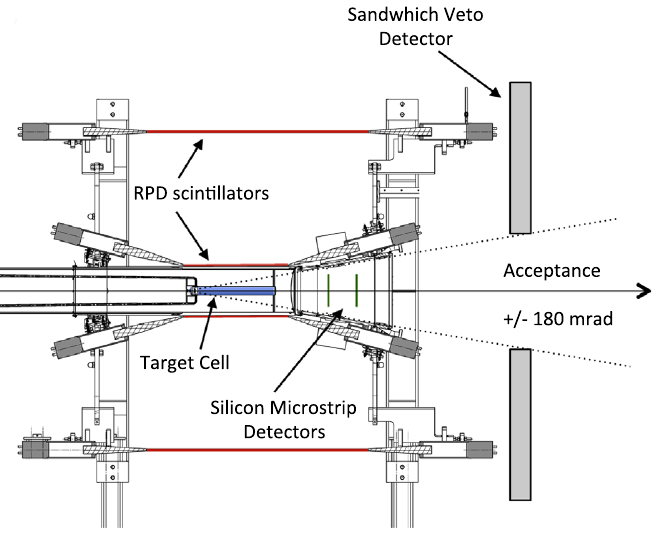
\includegraphics[width=0.5\textwidth]{sandwich}
	\caption{Scheme of detectors around the target region. The sandwich veto on the right prevent unmeasurable events with large scattering angles. Source: \cite{sandwich}}
	\label{fig:sandwich}
\end{figure}

The layout of COMPASS detectors is shown in figure \ref{fig:detec_layout}. Proton target is located inside the RPD (recoil-proton detector). On the left of target locate SciFi (scintillating fiber), BC (Beam counter) and silicon detectors. The coincidence of signals from SciFi and BC is used for the beam trigger, setting the time reference of whole system. The silicon detectors are applied for determining the location of projectile beam, which is further used to calculate the position of primary vertex. On the downstream very close to the target, there are sandwich veto and PixelGEM/Micromegas/DC (Pixel GEM detector, micromegas detectors and drift chamber). The function of sandwich veto is to reject the signal readout when the scattering polar angle of out-going particle is too large to measure. The structure of sandwich veto can be seen in figure \ref{fig:sandwich}, where the veto can be triggered if polar angle is out of acceptance. Behind the sandwich veto, PixelGEM/Micromegas/DC detectors are implemented to measure the angles of out-going particles with high accuracy and resolution. On the downstream further away from the target, two different sets of detectors are set up for measuring out-going particles with small and large scattering angles. 

The first set, located in the front, is used as large angle spectrometer (LAS). The major components of LAS are SM1 (solenoid magnet 1), tracking detectors, RICH (ring-image Cherenkov detector), ECAL1, HCAL1 and Muon filter. SM1 provides the magnetic field to deviate charged particles. The degree of deviation is measured by the tracking detectors on the both sides, which can calculate the momentum of out-going charged particles. The RICH detector on the right side on SM1 is used to improve the permanence of experiment by separating $\pi$ and $K$ in high intensity environment\cite{RICH}. ECAL1 is an electromagnetic calorimeter used to measure the energy of particles like electrons or photons while HCAL1, a hadron calorimeter, is used to measure the energy of hadron particles. Muon can be identified by tracking detectors behind a muon filter, which intercept every particles except muon.

The second set, located at the end of downstream, is deployed as small angle spectrometer (SAS). Most of its components have the same functionalities as their counterparts in LAS. The main additional detectors in SAS contains two BKs (beam killer), which are basically two scintillating counters. They are used to veto the non-interacting particle beams\cite{sandwich}.




